\documentclass[../thesis.tex]{subfiles}

\begin{document}

\chapter{Looking back, looking forward}%
\label{chap:pastAndFuture}

\section{History of neutrino oscillations}
\label{sec:history}

In the late 1960s, deep in the Homestake mine located in South Dakota, Ray Davis filled a large tank with tetrachloroethylene, a common dry-cleaning agent, and waited as solar neutrinos interacted with chlorine-37 atoms via the reaction
\begin{equation}
  \mathrm{\nu_e + \ ^{37}Cl \longrightarrow \ ^{37}Ar + e^-.}  
\end{equation}
Every few weeks, from 1970 to 1994, helium was bubbled through the liquid to extract the few dozen argon atoms that were produced in the time since the previous extraction. Each extraction was then placed in a gas-filled proportional chamber, where the $^{37}$Ar decays (roughly one per week) were counted over the course of a year or so (long enough to count effectively all of the atoms, given the 35-day half-life of $^{37}$Ar). By the early 1970s, the measurements were clearly indicating a reaction rate that was one-third of the prediction derived from the Standard Solar Model (SSM) \cite{DAVIS199413}. This ``solar neutrino problem'' was interpreted to mean that either the SSM or the experiment was in error, and neutrinos remained, according to the wisdom of the day, massless.

Despite the prevailing belief in masslessness, the possibility of massive neutrinos was considered as early as 1962, soon after the discovery that neutrinos come in separate electron and muon flavors. That year, in the ``MNS'' paper by Maki, Nakagawa, and Sakata \cite{10.1143/PTP.28.870}, the authors considered the possibility of neutrino flavor mixing, possibly from a nonzero mass. Neutrino mixing had been considered previously by Pontecorvo in 1957 \cite{Pontecorvo:1957cp}, but in the form of neutrino-antineutrino mixing, in analogy with the then-recently discovered phenomenon of neutral kaon mixing \cite{PhysRev.105.1925.2}. Pontecorvo revisited the subject in 1967, building upon the MNS formalism to describe how oscillations could occur in traveling neutrinos, going so far as to suggest that solar neutrinos could oscillate (well before the first experimental hints of such by the Davis experiment). Still, it would take decades of further observations to prove that these four theorists were correct.

The late 1980s delivered additional anomalies, when the Kamiokande \cite{HIRATA1988416} and IMB \cite{PhysRevLett.66.2561} experiments observed a deficit in the number of atmospheric charged-current \(\mathrm{\nu_\mu}\) events relative to expectations. In addition, Kamiokande also confirmed the solar neutrino problem \cite{SUZUKI199554}, which was yet again confirmed around 1992 by the gallium-based SAGE \cite{GAVRIN200136} and GALLEX \cite{VIGNAUD199820} radiochemical experiments. In 1996, the massive Super-Kamiokande (SK) water Cherenkov detector came online, and in 1998 the SK collaboration published measurements of the zenith angle dependence of the atmospheric neutrino deficit \cite{PhysRevLett.81.1562}. This geometric dependence was consistent with mass-induced flavor oscillations. Other models, such as neutrino decay or decoherence, were disfavored by the SK data, which was of sufficient quality to provide initial values of \(\theta_{23}\) and \(\Delta m^2_{32}\) (defined in \autoref{sec:oscPhysics}). Super-Kamiokande's compelling evidence in favor of nonzero neutrino mass would soon receive confirmation from other experiments.

Such confirmation arrived dramatically in 2002, thanks to the Sudbury Neutrino Observatory (SNO) \cite{PhysRevLett.89.011301}. Owing to its use of heavy water as the target material, SNO had unprecedented sensitivity to neutral current (NC) interactions, which are undergone by all three neutrino flavors. This NC sensitivity stood in addition to SNO's customary sensitivity to charged current (CC) interactions, which (at the relevant energy scale of $\sim$10~MeV) only provide detection of electron neutrinos. As such, SNO was capable of independently measuring both the total and the electron neutrino fluxes. The total flux was in excellent agreement with the SSM, demonstrating that the ``missing'' neutrinos underlying the solar neutrino problem were, in fact, merely hiding in the form of muon and tau neutrinos. SNO thus succeeded both in confirming the existence of neutrino mass and in resolving the solar neutrino problem, once and for all.

At this point, the existence of neutrino oscillations was no longer a question, but a fact. The precision era had begun, and the Japan-based reactor neutrino experiment KamLAND was one effort that had gotten a head start. KamLAND was initially proposed to search for potential oscillation in 1994, when the solar measurements were still murky, but by 1997 there was enough evidence from the results of Davis, SAGE, and GALLEX to suggest that KamLAND might be able to measure $\theta_{12}$ and $\Delta m^2_{21}$, if indeed such parameters were responsible for the solar neutrino deficit (and assuming that $\theta_{12}$ was sufficiently large, which remained an open question). Around the time of SNO's announcement, KamLAND published results on the disappearance of reactor antineutrinos over long ($\sim$100~km) baselines \cite{PhysRevLett.90.021802}. KamLAND succeeded in pinning down the value of $\theta_{12}$, in favor of the large mixing angle solution, and furthermore provided what remains the most precise measurement of \(\Delta m^2_{21}\) ever performed.

Meanwhile, the atmospheric results of SK and others on \(\Delta m^2_{32}\) had set off a flurry of successful long-baseline accelerator experiments, such as K2K \cite{PhysRevD.74.072003}, T2K \cite{ABE2011106}, MINOS \cite{PhysRevLett.101.131802}, NO$\nu$A \cite{PhysRevLett.123.151803}, OPERA \cite{Agafonova_2012}, and ICARUS \cite{Rubbia_2011}, optimized for this mass splitting and designed to narrow down its value and that of $\theta_{23}$. As the 2010s approached, however, one mixing angle remained elusive: $\theta_{13}$.

The disappearance of electron (anti)neutrinos is controlled by $\theta_{12}$ and \(\Delta m^2_{21}\) at longer baselines (such as those employed in solar neutrino experiments and KamLAND) and by $\theta_{13}$ and \(\Delta m^2_{31}\) at shorter baselines. As luck would have it, at the energies of reactor antineutrinos, the latter oscillation length is $\sim$1~km, which is a sufficiently short distance that a relatively modest target mass of $\sim$10~tons will provide ample statistics from a typical commercial power reactor. By adopting such baselines and target masses, the Chooz experiment in France, as well as the Palo Verde experiment in the USA, set the stage for the reactor-based study of neutrino oscillations. Unfortunately, for Chooz and Palo Verde, sensitivity to oscillations was limited, in large part due to the dependence of a single-detector configuration on modeling the absolute reactor antineutrino flux.\footnote{Rapid deterioration of the gadolinium-doped scintillator was another obstacle.} These two experiments were unable to discover evidence of oscillation, instead setting upper limits of roughly $\sin^2 2\theta\,<\,0.17$ (for a mass-squared splitting of $|\Delta m^2_{32}| \approx 2.5\times10^{-3}\,\text{eV}^2$). Importantly, however, this result excluded $\nu_\mu \rightarrow \nu_e$ oscillations as the driver of the atmospheric $\nu_\mu$ disappearance seen by experiments such as Super-K.

In order to mitigate the uncertainty arising from modeling of the absolute antineutrino flux, the subsequent generation of reactor experiments were designed using identical detectors at different baselines \cite{Mikaelyan:1998yg}. This would enable the near detectors to measure the antineutrino flux while the far detectors measure any oscillation. Uncertainties on the absolute flux and detection efficiency thus largely cancel in the far/near ratio. The Double Chooz \cite{Ardellier:2006mn}, RENO \cite{Ahn:2010vy}, and Daya Bay \cite{Guo:2007ug} experiments embarked on this effort in parallel.


\section{History of reactor neutrino experiments}
\label{sec:introReactor}

Although a number of reactor-based experiments were briefly described in \ref{sec:history}, the history of the field merits further discussion, given that this thesis is based on one such experiment. Nuclear reactors have played an important role in experimental neutrino physics since the very beginning. Indeed, the Savannah River reactor provided the antineutrinos that led to the first direct confirmation of the particle's existence by the 1956 Cowan-Reines experiment. Since then, reactors have continued to provide key insights into the nature of the neutrino.

Essentially all reactor neutrino experiments are based on detecting charged-current inverse beta decay (IBD) interactions in a volume of liquid scintillator, observed by photomultiplier tubes. The details of this measurement principle are discussed in \autoref{chap:experim}. Among its advantages are (a) the fact that the double-pulse signature allows efficient background rejection without the need to evade cosmogenic backgrounds by going deep underground (especially important at km and shorter baselines, where a deep overburden would create challenging logistics), (b) the threshold energy is lower compared to a water Cherenkov detector, and (c) the materials and technology are inexpensive in comparison to advanced designs such as noble liquid time projection chambers. These advantages have remained pertinent from the Cowan-Reines experiment up to the present day.

Efforts involving reactor neutrinos gained steam in the 1970s, when interest arose in going beyond merely using nuclear reactors to qualitatively confirm the neutrino's existence and interactions. One of the new goals was to quantitatively measure the flux and spectrum of electron antineutrinos produced by nuclear reactors. These efforts bore fruit in the early-to-mid 1980s when a half-dozen experiments\footnote{ILL, Gosgen, Rovno, Krasnoyarsk, Bugey, and Savannah River.} published such measurements \cite{PhysRevD.24.1097,Zacek:1986cu,Afonin:1985rw,Aleshin_2008,Abbes:1995nc,Sobel:1982gf}. These early detectors were relatively small, with target masses of a few hundred kg (versus Daya Bay's 80~t at the far site); hence, short baselines (of 10--100~m) were necessary in order to obtain sufficient statistics. The fluxes measured by these experiments were in good agreement with the predictions of the ILL-Vogel model \cite{SCHRECKENBACH1985325,VONFEILITZSCH1982162,HAHN1989365,PhysRevC.24.1543}, which was developed around the same time. Much later, as discussed in \autoref{chap:reactor}, these measurements would provide evidence of the so-called reactor antineutrino anomaly \cite{PhysRevD.83.073006} associated with the Huber-Mueller reevaluations of the predicted flux \cite{PhysRevC.84.024617,PhysRevC.83.054615}, which lie $\sim5$\% higher than the measured fluxes. In addition, the data from one of these experiments (Bugey-3) would later be combined with Daya Bay's in order to set limits on light sterile neutrino mixing \cite{PhysRevLett.117.151801}.

The 1990s brought the Chooz \cite{Apollonio_2003} and Palo Verde \cite{PhysRevD.64.112001} experiments (mentioned previously in the context of neutrino oscillations), which employed larger, $\mathcal{O}$(10~t) detectors so as to acquire useful statistics at longer (km-scale) baselines. Although the search for oscillations was their primary goal, these two experiments were also able to measure the $\nubar_e$ flux at these longer baselines, comparable to the average baseline for the Daya Bay far site. 
% \footnote{XXX When was it fully confirmed that $\nu_\mu \rightarrow \nu_\tau$ was the explanation, rather than $\nu_\mu \rightarrow \nu_s$?}
As with the short-baseline experiments, Chooz and Palo Verde would later indicate a $\sim5$\% deficit with respect to the Huber-Mueller flux predictions.

The $\theta_{13}$ sector is not the only one in which reactor antineutrinos can play a useful role. The KamLAND experiment used reactors to confirm and complement the solar neutrino results on $\theta_{12}$ and $\Delta m^2_{21}$, significantly improving the precision on the latter. Located a kilometer underground in Japan's Kamioka mine, in the cavern formerly occupied by the Kamiokande-II detector, KamLAND employed a massive, transparent balloon filled with 1000~t of liquid scintillator \cite{PhysRevLett.90.021802}. Antineutrinos arrived from some 50 reactors scattered throughout Japan, at a flux-averaged baseline of 180~km. This $L/E$ was well-suited for measuring oscillations driven by $\Delta m^2_{21}$, and KamLAND's measurement of this splitting will remain unchallenged for the foreseeable future.
% Unrelated to reactor neutrinos, KamLAND was also the first experiment to observe \emph{geoneutrinos} \cite{kamlandGeo}, that is, antineutrinos produced by the decay chains of $^{238}$U and $^{232}$Th in the Earth.

Returning to the topic of $\theta_{13}$, in 1998, Mikaelyan and Sinev \cite{Mikaelyan:1998yg} rigorously showed that a two-detector (near and far) reactor experiment could overcome the absolute flux uncertainty and allow for precision measurement of $\sin^2 2\theta_{13}$. Although beam experiments also carry the potential to measure $\theta_{13}$ by observing $\nu_\mu \to \nu_e$ oscillation, they are susceptible to degeneracies between it and other parameters, such as the mass hierarchy, $\dcp$, and the other mixing angles. Reactors thus remained a favorable means to a pure $\theta_{13}$ measurement, despite the fact that disappearance channels are generally more challenging than appearance channels when measuring a small mixing angle.

Accordingly, in the mid-2000s, the Double Chooz \cite{Ardellier:2006mn}, RENO \cite{Ahn:2010vy}, and Daya Bay \cite{Guo:2007ug} experiments were proposed. All three shared the same basic design: Near and far detectors at a $\mathcal{O}$(1 km) (far) baseline, using gadolinium-doped liquid scintillator to improve detection efficiency and background rejection. In April 2011, Double Chooz began taking far site data, followed in August by RENO's full configuration, and in December by Daya Bay using a six-detector configuration. In March 2012, with just 55 days of data, Daya Bay announced a $5.2\sigma$ discovery of nonzero $\theta_{13}$ \cite{PhysRevLett.108.171803}, which was quickly confirmed by RENO in the following weeks \cite{PhysRevLett.108.191802}. Since then, these experiments have continued to publish increasingly precise measurements of $\theta_{13}$ and $\Delta m^2_{ee}$, as well as measurements of the absolute flux (confirming the anomaly) \cite{PhysRevD.100.052004,Atif:2020eyo,DoubleChooz2020}, the spectrum (discovering an as-yet unexplained excess of events around 5~MeV, relative to predictions) \cite{PhysRevD.100.052004,Atif:2020eyo,DoubleChooz2020}, and, at least in the case of Daya Bay, the time evolution of the flux and spectrum \cite{PhysRevLett.118.251801}, the decomposed fuel isotope components of the flux and spectrum \cite{PhysRevLett.123.111801}, sterile neutrino limits \cite{PhysRevLett.117.151801}, decoherence limits \cite{DayaBayWavePacket}, and numerous other valuable results, demonstrating the major scientific utility of reactor neutrino experiments.

Recent years have seen a resurgence of activity in short-baseline ($\sim$5--25~m) reactor experiments, motivated both by the need for precise measurement of the reactor antineutrino flux/spectrum as well as by the prospect of an eV-scale sterile neutrino (as suggested, controversially, by the reactor antineutrino anomaly \cite{PhysRevD.83.073006}, the SAGE/GALLEX anomalies \cite{PhysRevC.80.015807,KAETHER201047}, and the anomalous $\nu_e$ results of the LSND and MiniBooNE accelerator experiments \cite{PhysRevD.64.112007,PhysRevLett.121.221801}). These ton-scale experiements\footnote{Among them, NEOS \cite{Ko:2019cip}, DANSS \cite{Alekseev_2016}, STEREO \cite{Allemandou_2018}, PROSPECT \cite{ASHENFELTER2019287}, NEUTRINO-4 \cite{Serebrov:2020kmd}, and SoLiD \cite{Abreu_2021}} complement each other with different reactor types (commercial or research), baselines/mobility, scintillator materials (liquid or plastic), neutron capture isotopes (Gd or $^6$Li), and levels of segmentation (3D, 2D, or none). With the exception of SoLiD, all of these experiments have already published valuable results, including new limits on sterile neutrino mixing around 1~eV$^2$ \cite{PhysRevLett.118.121802,Svirida:2019kbq,PhysRevD.102.052002,PhysRevD.103.032001}, strong rejection of sterile neutrinos as the explanation of the reactor antineutrino anomaly \cite{PhysRevD.102.052002,PhysRevD.103.032001}, confirmation of the 5~MeV bump \cite{PhysRevLett.118.121802}, and precise measurement of nearly-pure antineutrino spectra from $^{235}$U \cite{PhysRevD.103.032001}. Intriguingly, NEUTRINO-4 has claimed to observe $4.6\sigma$ evidence for sterile neutrino mixing at a $\Delta m^2$ of 7.25~eV$^2$ \cite{Serebrov_2020}, but time will tell whether this is borne out by other experiments.

Finally, looking to the future, the 20~kt JUNO detector \cite{juno} (in southern China) will be by far the largest reactor neutrino detector ever constructed. The driving goal of the JUNO experiment is the determination of the mass hierarchy (see \autoref{sec:majorana}) without susceptibility to the degeneracies and correlations that complicate the hierarchy determination in accelerator experiments \cite{Ghosh:2017sli}. JUNO will observe $\nubar_e$ interactions using more efficient PMTs and significantly larger photocathode coverage in order to achieve sub-3\% energy resolution. At this resolution, the two hierarchies produce measurable differences in the high-frequency oscillations due to $\theta_{13}$ of the $\nubar_e$ spectrum. If JUNO is successful, it could determine the mass hierarchy years before other (beam-based) experiments are expected to do so, cementing yet another historical achievement for the humble reactor antineutrino.

\section{Relevance of $\theta_{13}$ to future research}
\label{sec:futureRelevance}

Quantitatively, the value of $\theta_{13}$ is broadly useful in the context of beyond-the-Standard-Model (BSM) model building. More concretely, however, $\theta_{13}$ is important in the context of unraveling two extremely significant properties of neutrinos: The value of $\dcp$, and the mass hierarchy (MH). In this context, the importance of $\theta_{13}$ arises simply from the fact that $\dcp$ and the MH both influence oscillation probabilities via higher-order terms that are controlled by e.g. \(\sin^2\theta_{13}\) or \(\sin^2 2\theta_{13}\); thus, a larger $\theta_{13}$ (up to a certain point) implies a greater experimental sensitivity to these subtle effects. In turn, $\dcp$ and the MH are pivotal in relation to two of the biggest questions in particle physics: The origin of the the matter-antimatter asymmetry of the Universe, and the Majorana nature (or lack thereof) of the neutrino, respectively.

\subsection{Baryon asymmetry and $\dcp$}
\label{sec:baryonAsym}

Most physical processes produce, in aggregate, equal amounts of matter and antimatter. And yet, our present universe contains a clear excess of matter. The origin of this excess thus demands our investigation. Although the specific mechanisms at play remain unknown, together they must fulfill the \emph{Sakharov conditions.} As most of the normal matter in the Universe is baryonic, explaining the matter-antimatter asymmetry largely boils down to explaining \emph{baryogenesis,} the generation of excess baryons over antibaryons. The three Sakharov conditions, in the context of baryogensis, are:

\begin{enumerate}
\item Existence of processes that violate baryon number symmetry $B$; otherwise, every baryon would be created in concert with an antibaryon
\item Existence of processes that violate C and CP symmetry; otherwise the C and CP-conjugates of $B$-violating interactions would cancel out the asymmetry
\item Lack of thermal equilibrium (at some point in history); otherwise, every process would be counterbalanced by its CPT-conjugate
\end{enumerate}

Within the SM, an asymmetry can theoretically be produced via the mechanism of electroweak baryogenesis. However, the only source of CP violation in the SM is the complex phase in the CKM matrix, and it is known that this effect alone is not large enough to account for the observed matter-antimatter asymmetry \cite{Shaposhnikov:2009zzc}. If the neutrino $\dcp$ is found to deviate significantly from zero (or $\pi$), then this would constitute a brand new source of CP violation, and if the effect is large enough, it could fully explain our matter-dominated universe (when harnessed by a BSM mechanism such as leptogenesis). Thus, $\dcp$, in a sense, could play a critical role in explaining why the universe is not a formless sea of photons. Conversely, if it is found to be small or consistent with zero, then the mystery of baryogenesis will be deepened even further. For these reasons, the measurement of $\dcp$ is a chief driving goal of some of the most ambitious neutrino oscillation experiments underway. This effort would be far more difficult if Nature had chosen a much smaller $\theta_{13}$.

\subsection{Majorana neutrinos and the mass hierarchy}
\label{sec:majorana}

As is illustrated in \autoref{fig:massOrdering}, the ordering of the neutrino masses is not fully known. Determining the mass hierarchy is an important effort in its own right. The MH affects cosmological models, kinematic measurements of the neutrino mass,
% (XXX is this true???),
the measurement of $\dcp$, and BSM model building, to name a few examples of its importance. It even relates to the question of the very nature of the neutrino mass, as we show here.

In the SM, the neutrino is a simple two-component left-handed \emph{Weyl} spinor. Once mass is added, however, the picture necessarily becomes more complicated. Massive spinors can be classified as either of Majorana or Dirac type. A Majorana spinor is, by definition, one that is invariant under the operation of charge conjugation (i.e., it is identical to its antiparticle). A Dirac spinor, on the other hand, is not self-conjugate, and contains twice as many components.

For a Majorana spinor, the Hamiltonian can contain a term (the Majorana mass) that contributes to the particle's mass and creates particle-particle pairs. Obviously, this is impossible if the particle carries any sort of conserved charge, as is the case for every particle of the SM, except (after electroweak symmetry breaking) the neutrino. Thus, the neutrino could prove to be the first known fundamental Majorana fermion, and if this is so, it would also provide the first example (via the Majorana mass) of lepton number violation.

The possible Majorana nature of the neutrino is closely related to the question of the smallness of the neutrino mass scale. Taking a step back, the simplest model of neutrino mass (which furnishes Dirac neutrinos) can be constructed in analogy with the masses of the other fermions: We introduce a sterile $\nu_{\text{R}}$ and construct a Yukawa coupling between it, the Higgs field, and the active $\nu_{\text{R}}$. The lack of a Majorana mass term means that $\nu_{\text{R}}$ and $\nu_{\text{L}}$ can be combined into a single Dirac spinor. Although this construction works, it suffers from the fact that the dimensionless coupling constant must be extremely small, of order $m_\nu/m_{\text{EW}}$.

An alternative (and generally more favored) model of neutrino mass is described by the \emph{seesaw mechanism}. In this case, sterile right-handed neutrino fields $\nuR$ are introduced, self-coupled via Majorana mass term near the GUT scale. (Such Majorana masses are not allowed for the fundamental $\nuL$ fields as they carry weak hypercharge.) In addition, Dirac mass terms are introduced, linking $\nuR$ and $\nuL$ at the electroweak scale. The resulting mass matrix contains three small and three large eigenvalues, with the small ones being of the order \(m^2_{\text{EW}} / m_{\text{GUT}}\). The corresponding eigenstates behave as Majorana particles: They are self-conjugate, and they have a Majorana mass term (leading to $L$ violation). This model thus naturally generates small neutrino masses. Furthermore, the heavy sterile neutrinos are a fairly generic prediction of GUT and other BSM theories. Finally, even more generic higher dimensional operators can also be shown to generate Majorana mass terms in the effective low-energy theory. For these reasons, the theory community regards Majorana neutrinos as a likely fact of nature. The experimental challenge is then to find experimental evidence of the Majorana neutrino.

The hypothetical process of neutrinoless double beta decay ($\ndbd$) holds the key to potentially observing evidence of Majorana neutrinos. In ordinary double beta decay, an isotope emits two electrons and two antineutrinos. A Majorana mass would allow the two antineutrinos to ``annihilate'', leading to a small peak at the endpoint of the double beta spectrum. If this peak is observed, it would constitute definitive evidence of the Majorana nature of the neutrino, with profound implications for BSM model building.

The rate of $\ndbd$ is proportional to the square of the \emph{effective Majorana mass} of the electron neutrino,
\begin{equation}
  m_{\beta\beta} \equiv \left| \sum m_i U^2_{ei} \right|,
  \label{eq:majoranaEffMass}
\end{equation}
in which the unknown Majorana phases of the $U_{ei}$ can interfere with each other. It turns out that the mass hierarchy has important implications when it comes to the range of possible values of $m_{\beta\beta}$. For a given hierarchy, the three neutrino masses are uniquely determined by the mass $m_l$ of the lightest one, since the values of $\Delta m^2$ are known. Then, for a given $m_l$ (and hierarchy), the possible range of $m_{\beta\beta}$ is determined by varying the three Majorana phases. For $m_l$ above $\sim0.1$~eV, the two hierarchies give largely the same $m_{\beta\beta}$ ranges. However, at lower $m_l$ the two hierarchies differ considerably. In the case of the inverted hierarchy, $m_{\beta\beta}$ remains above $\sim0.01$~eV for all $m_l$. On the other hand, under the normal hierarchy, the Majorana phases can cancel completely when $m_l$ is between $\sim2$ and 8~meV (making $\ndbd$ unobservable). Below 2~meV, $m_{\beta\beta}$ is bounded from below, but its range lies an order of magnitude below that for the IH case. See \autoref{fig:doublebeta}.

\begin{figure}[h]
  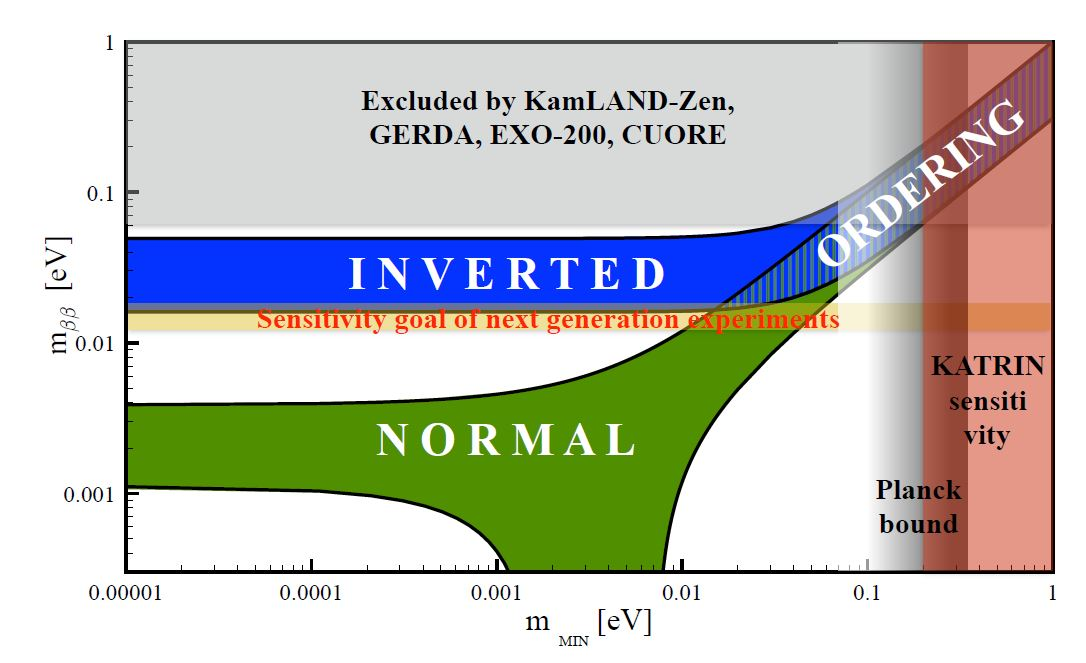
\includegraphics[scale=0.75]{doublebeta.jpg}
  \caption{The dependence of the effective Majorana mass $\abs{m_{\beta\beta}}$ on the minimum neutrino mass $m_{\mathrm{MIN}}$. From \cite{giuliani2020double}.}
  \label{fig:doublebeta}
\end{figure}


The upcoming generation of $\ndbd$ experiments seek to probe the entire range of $m_{\beta\beta}$ values allowed by the inverted hierarchy. Therefore, \emph{if it is established that the mass ordering is inverted,} then a null result from these $\ndbd$ experiments would demonstrate conclusively that \emph{the neutrino is not a Majorana particle.}\footnote{At least if there are no sterile neutrinos.} Meanwhile, if the normal hierarchy is confirmed, then it becomes impossible to disprove the Majorana nature of the neutrino, since it may be hiding beneath a very small value of $m_{\beta\beta}$. (Of course, proving, as opposed to disproving, the Majorana nature remains possible via observation of $\ndbd$.) The mass hierarchy thus is extremely relevant to the task of determining the nature of neutrino mass, and, in turn, the large value of $\theta_{13}$ makes it possible to determine the MH via oscillation experiments. As shown by \autoref{eq:majoranaEffMass}, $\theta_{13}$ also plays an important role in the relation between $m_{\beta\beta}$ and the physical masses $m_i$.

Furthermore, as was mentioned earlier, the determination of the mass hierarchy would carry significant implications for the measurement of $\dcp$. Many experiments in the pipeline, particularly those that take advantage of matter effects, suffer from a degeneracy between $\dcp$ and the mass hierarchy, forcing them to quote two, possibly very different, confidence intervals for $\dcp$. The result is a considerably reduced overall sensitivity to leptonic CP violation. Knowledge of the hierarchy would eliminate this issue. With the knowledge that $\theta_{13}$ is large, measuring the mass hierarchy is an easier prospect in general, but in particular it allows for experiments, such as JUNO, that aim to efficiently determine the MH independently of $\dcp$. This accelerates the timeframe of MH determination, while also providing improved sensitivity to long-term $\dcp$(+MH) experiments such as DUNE and Hyper-Kamiokande. $\theta_{13}$, via its connection to the mass hierarchy, thus also provides an indirect boost to the $\dcp$ measurement effort, in addition to its direct influence on the oscillation probability.


\end{document}